% Drawing 69/01-14 -- folder 69, batch 01, archive page 16 (PDF page 17).
% Transcription: un petit triangle ; à côté, un graphe à quelques sommets entouré de deux ovales qui se croisent ; plus bas, une étoile à trois branches dont chaque bout porte un petit triangle (deux sommets reliés au bout de la branche)
% Kind: small triangle, graph in two ovals, star of triangles. Method 2 (schematic redraw from the facsimile). Status: partial.
% Notes: A small triangle; beside it a graph on seven vertices (three of them inked heavy) inside two crossing closed curves; below, the 'star': a central triangle whose three vertices each carry two narrow spikes, each spike a small triangle (two vertices joined to the vertex of the central triangle, one of them often a heavy dot). The vertices are placed once and every edge runs between them, so the spikes close exactly. Still differs from the facsimile: the edges of the graph inside the ovals are a reading of short overlapping strokes; the two closed curves are approximate. The description's 'three-branch star' is on the page a central triangle with six spikes (two at each vertex). Redrawn 2026-11-09 (issue 128): vertices placed once and every edge drawn between them, labels at \small, strike-outs not drawn; to check again.
% Coordinates: 1 unit = 1 mm = 1/100 of the crop width (bbox in page fractions: [0.12, 0.3, 0.36, 0.5]).
% Redrawn by Claude (claude-opus-5-5), issue #73, 2026-11-09; not checked by a human; not compiled (no TeX in the session).
% Rights: reproduces part of the work -- behind RENDER_TRANSCRIPTS, never published by itself.
\documentclass[tikz,border=3pt]{standalone}
\usepackage{amsmath,amssymb}
\usetikzlibrary{patterns,arrows.meta}
\tikzset{pencil/.style={black!45}, struck/.style={black!35}, mark/.style={circle,draw,inner sep=1.3pt}, pt/.style={circle,fill,inner sep=0.9pt}, opt/.style={circle,draw,fill=white,inner sep=1.1pt}}
\begin{document}
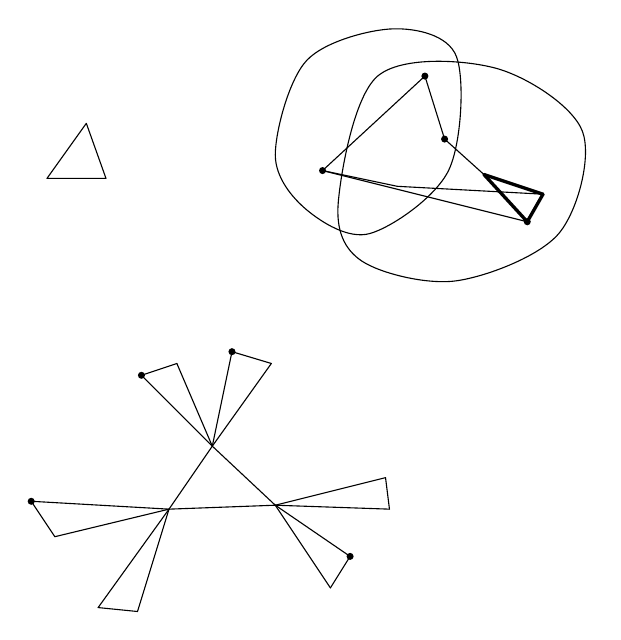
\begin{tikzpicture}[x=1mm,y=1mm,line cap=round,line join=round,font=\scriptsize]
\draw (26,-34) -- (21,-41) -- (28.5,-41) -- cycle;
\draw plot[smooth cycle, tension=0.55] coordinates {(50,-38) (54,-26) (65,-22) (73,-25.5) (72,-40) (62,-48) (54,-45)};
\draw plot[smooth cycle, tension=0.55] coordinates {(63,-28) (78,-27) (89,-35) (86,-48) (73,-54) (61,-51.5) (58,-44)};
\draw (69,-28) -- (56,-40);
\draw (69,-28) -- (71.5,-36);
\draw (71.5,-36) -- (76.5,-40.5);
\draw (56,-40) -- (65.5,-42);
\draw (65.5,-42) -- (84,-43);
\draw (56,-40) -- (82,-46.5);
\draw[very thick] (76.5,-40.5) -- (84,-43);
\draw[very thick] (84,-43) -- (82,-46.5);
\draw[very thick] (76.5,-40.5) -- (82,-46.5);
\node[pt] at (69,-28) {};
\node[pt] at (56,-40) {};
\node[pt] at (82,-46.5) {};
\node[pt] at (71.5,-36) {};
\draw (42,-75) -- (36.5,-83);
\draw (42,-75) -- (50,-82.5);
\draw (36.5,-83) -- (50,-82.5);
\draw (42,-75) -- (33,-66);
\draw (42,-75) -- (37.5,-64.5);
\draw (33,-66) -- (37.5,-64.5);
\node[pt] at (33,-66) {};
\draw (42,-75) -- (44.5,-63);
\draw (42,-75) -- (49.5,-64.5);
\draw (44.5,-63) -- (49.5,-64.5);
\node[pt] at (44.5,-63) {};
\draw (36.5,-83) -- (19,-82);
\draw (36.5,-83) -- (22,-86.5);
\draw (19,-82) -- (22,-86.5);
\node[pt] at (19,-82) {};
\draw (36.5,-83) -- (32.5,-96);
\draw (36.5,-83) -- (27.5,-95.5);
\draw (32.5,-96) -- (27.5,-95.5);
\draw (50,-82.5) -- (64,-79);
\draw (50,-82.5) -- (64.5,-83);
\draw (64,-79) -- (64.5,-83);
\draw (50,-82.5) -- (59.5,-89);
\draw (50,-82.5) -- (57,-93);
\draw (59.5,-89) -- (57,-93);
\node[pt] at (59.5,-89) {};
\end{tikzpicture}
\end{document}
